\section{Reconstruction-aware sensor layout}
\label{sec:problem}

Let $G=(\calV,E)$ denote a traffic network with candidate sensing locations $\calV$. At each time $t$, the traffic state is $x_t \in \R^{|\calV|}$. A deployment chooses a fixed sensor set $\calS \subseteq \calV$ with $|\calS| \leq k$ and observes $x_{t,\calS}$, while the hidden complement $\calH=\calV\setminus\calS$ must be reconstructed. The design objective is not to recover an OD matrix or guarantee full observability; it is to choose $\calS$ so that a transparent reconstruction rule $\hat{x}_{t,\calH}=f_{\calS}(x_{t,\calS})$ has low held-out error on hidden components.

\begin{definition}[Budgeted hidden-network reconstruction design]
Given a candidate set $\calV$, a sensor budget $k$, a training split $\calD_{\mathrm{tr}}$, selector-validation split $\calD_{\mathrm{sel}}$, tuner-validation split $\calD_{\mathrm{tun}}$, test split $\calD_{\mathrm{te}}$, and a transparent reconstruction family $\{f_{\calS}:|\calS|\le k\}$, the design problem is to output a fixed layout $\hat{\calS}$ before test evaluation so that hidden-component deployment risk
\[
    R(\calS)=\E\!\left[\ell\!\left(x_{\calH}, f_{\calS}(x_{\calS})\right)\right],
    \qquad \calH=\calV\setminus\calS,
\]
is small for a reconstruction loss $\ell$. The empirical paper metric uses hidden-component MAE on $\calD_{\mathrm{te}}$ after $\hat{\calS}$ and all layout-selection rules are fixed.
\end{definition}

The experiments use transparent GLS/MAP and graph-signal reconstruction models. Training data estimate reconstruction ingredients such as means, covariances or precisions, graph operators, shrinkage levels, and regularization. Selector-validation data choose the best layout within each candidate scoring rule. Tuner-validation data choose the scoring rule or score vector. Test data are used only after the layout rule is fixed. This split discipline prevents validation reconstruction error from being treated as final deployment evidence.

\begin{figure}[t]
\centering
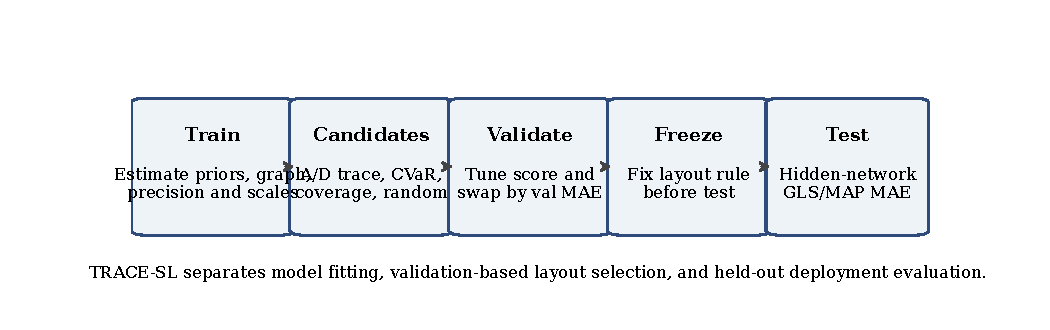
\includegraphics[width=\textwidth]{figures/fig1_workflow.pdf}
\caption{TRACE-SL workflow. The design protocol separates training-derived reconstruction ingredients, validation-based layout selection, and held-out deployment evaluation.}
\label{fig:workflow}
\end{figure}

For a candidate layout $\calS$, the primary test metric is hidden-component MAE,
\[
    \mathrm{MAE}(\calS)=\frac{1}{|\calT_{\mathrm{test}}||\calH|}
    \sum_{t\in\calT_{\mathrm{test}}}\|x_{t,\calH}-\hat{x}_{t,\calH}\|_1.
\]
The paper-source artifacts also report RMSE, MAPE where available, posterior trace, condition number, log determinant, scenario CVaR trace, coverage, and validation diagnostics. The central claim is empirical and scoped: layouts selected by TRACE-SL improve reconstruction in the tested settings and under the stated transparent reconstruction protocol.

This formulation deliberately keeps the target narrower than complete network observability. A layout may fail to identify every latent path or OD flow and still be useful for hidden-state recovery if it improves the reconstruction loss of the traffic state variables actually used by the downstream estimator. Conversely, a layout with strong topological coverage can be weak under the held-out reconstruction metric if the observed locations are redundant for the temporal-spatial variation in the hidden complement.
